\documentclass[a4paper, twocolumn]{article}


% you can switch between these two (and more) styles by commenting one out (use percentage)
\usepackage[backend=biber]{biblatex}
%\usepackage[backend=biber, style=authoryear-icomp]{biblatex}
\addbibresource{./refs.bib}

\usepackage{graphicx}

\usepackage{listings}
\usepackage{color}
\definecolor{lightgray}{gray}{0.9}

% code listing: https://tex.stackexchange.com/questions/19004/how-to-format-an-inline-source-code
\lstset{
    showstringspaces=false,
    basicstyle=\ttfamily,
    keywordstyle={blue},
    commentstyle=\color[gray]{0.6}
    stringstyle=\color[RGB]{255, 150, 75}
}
\newcommand{\inlinecode}[2]{\colorbox{light gray}{\lstinline[language=#1]$#2$}}

\author{Jeffrey Roed, Joachim Richter, and Rasmus Kibshede}
\title{Predicting Car Mileage and Make using Linear and Logistic Regression}



\begin{document}


\twocolumn[
    \begin{@twocolumnfalse}
        \maketitle
        \begin{abstract}
            The findings reveal that accurate prediction of car mileage and make is achievable using machine learning models. Key predictors such as engine displacement, horsepower, and origin significantly influence the outcomes. The best-performing models exhibit high accuracy and provide valuable insights into the relationships between predictor variables and target outcomes.
        \end{abstract}
    \end{@twocolumnfalse}
    \vspace{1cm}
]


\section{Introduction\label{sec:Introduction}}
Group name: Silicon\\
Predictive modeling in the automotive industry has become increasingly relevant and valuable in recent years, offering insights into vehicle performance, efficiency, and market trends. In this study, we address two fundamental questions \ref{sec:Research Question}
 
These questions drive our investigation into the predictive capabilities of machine learning models when applied to a dataset comprising detailed information about automotive performance and specifications. By exploring these questions, we aim to assess the feasibility and accuracy of leveraging predictive analytics techniques, particularly linear regression for mpg prediction and logistic regression for make prediction. Our findings have the potential to contribute valuable insights to the automotive industry, informing decisions related to vehicle design, marketing strategies, and consumer preferences.


% The introduction must put your paper into a context.
% The reader should be able to understand your paper based on the background information provided in the introduction.

\section{Research Question\label{sec:Research Question}}
Q1: Is it possible to predict the outcome of a car's miles per gallon (mpg) based on various factors such as the number of cylinders, displacement, horsepower, weight, acceleration, model year, origin, make and model?\\
Q2: Is it possible to predict a car's make based on the same factors?

% The research question must be phrased as a question, ending with "?".
% It is often a good idea to structure your research question into one overall question with a number of sub-questions, and you can number them i.e. Q1, Q2 etc. to make it easy to refer to them.
% Alternatively, you can phrase a hypothesis instead of a research question.

\section{Methods\label{sec:Methods}}

A correlation matrix was created after cleaning up the dataset. This matrix showed a strong negative linear relationship between mgp, cylinders, displacement, horsepower, and weight. This enabled the study to move forward with the hypothesis that we could determine mgp based on our dataset. 

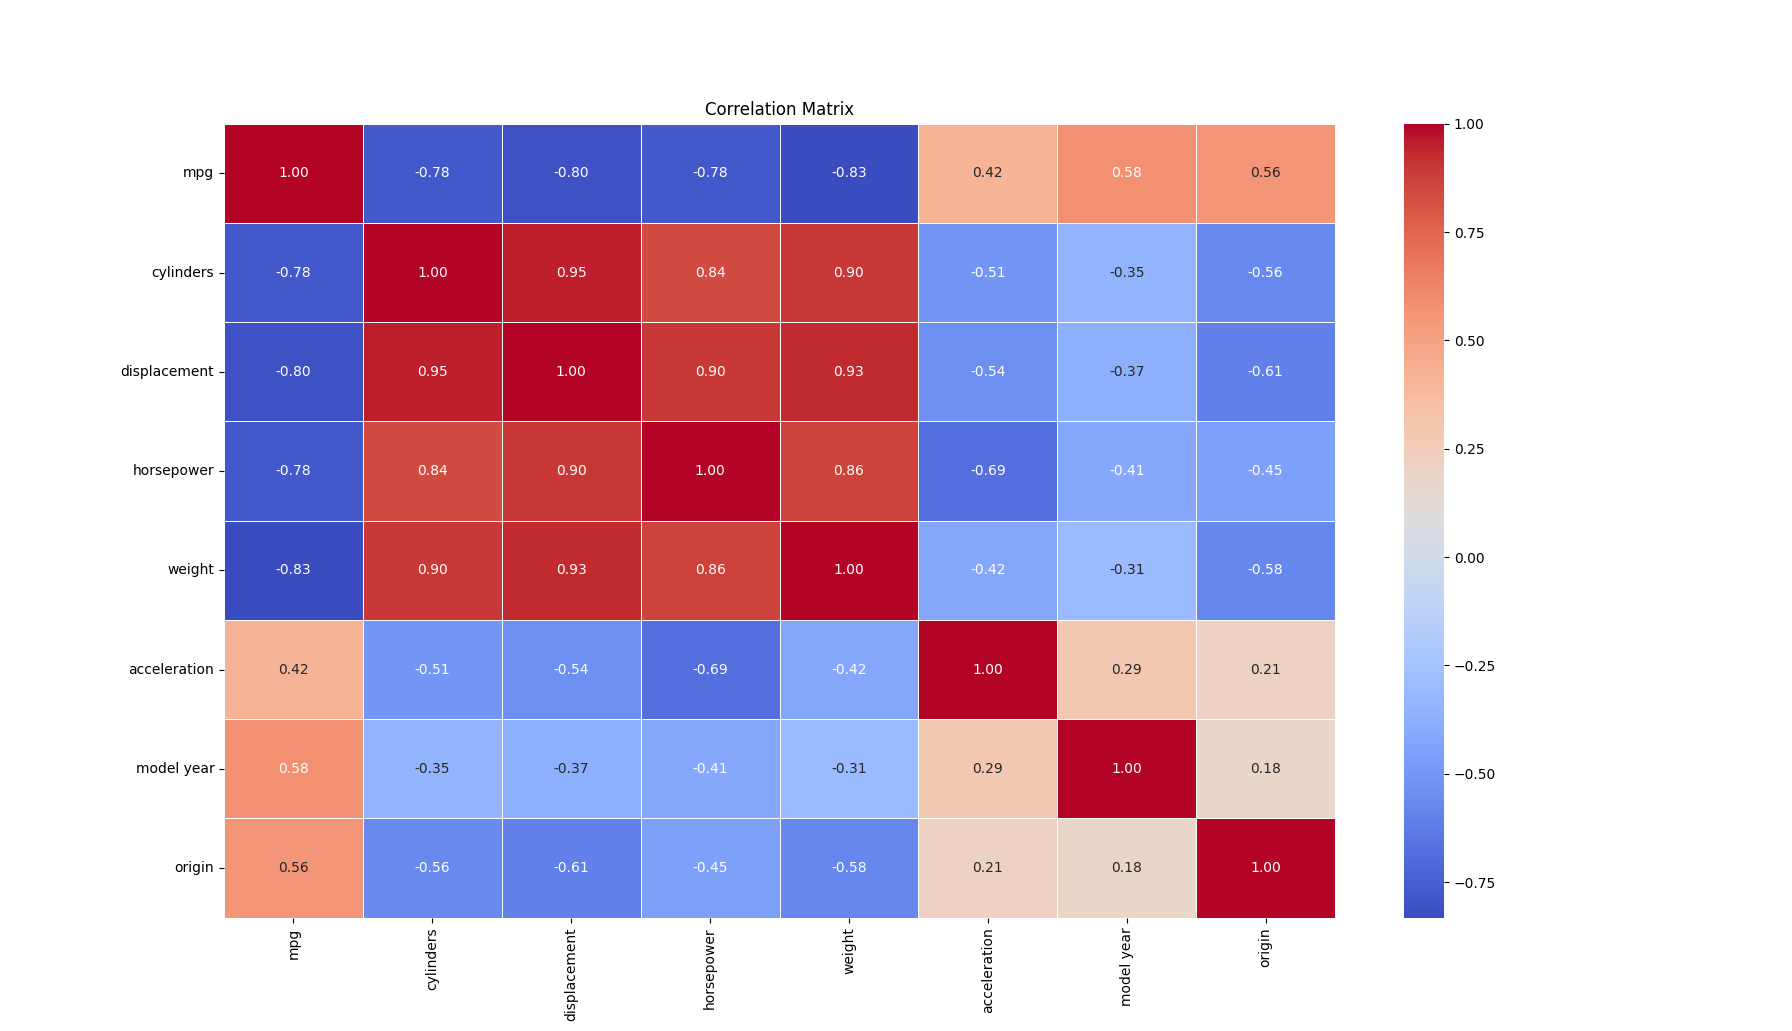
\includegraphics[width=0.9\linewidth]{images/Correlation.png}


In this study, linear regression and logistic regression were applied to predict the outcome of a car's miles per gallon and make, respectively. Linear regression utilized factors such as the number of cylinders, displacement, horsepower, weight, acceleration, model year, origin, and car name to predict miles per gallon. Logistic regression used the same factors to predict the car's make.

The dataset, provided by Henrik Strøm, an AI teacher at KEA, included details on car performance and make. Initial examination revealed faulty and deficient data. Using well know data cleaning techniques such as Preprocessing \textcite{hellerstein2013quantitative}

Following the data completion, feature engineering was conducted. This process transformed categorical variables, such as make and model, into numerical values through the use of one-hot encoding, enabling their inclusion in the regression analysis.

Different machine learning models were considered, and their performances were gauged using metrics such as mean squared error, mean absolute error, and root mean squared error.

The data was split into three data groups for training, validation, and testing. The training set was used to fit the models, the validation set was used for model selection and tuning, and the testing set was used to evaluate the performance of the final selected model.

% The methods section is for documenting the methods you apply to conduct your research.
% It is about the methods and how they will be applied, but not about their actual application.
% Ideally, you should write your method section before you start the actual research.
% The methods section must be well referenced.

\section{Analysis\label{sec:Analysis}}

Exploratory data analysis was conducted to uncover insights into the connections between predictor variables and the target outcomes, which are miles per gallon (mpg) and car make. Using descriptive statistics, visualizations, and correlation analysis, this phase explored the data to understand its distribution, identify patterns, and reveal associations between variables. Subsequently, the performance of each machine learning model was scrutinized to determine how well it could predict the car's mpg and make. The accuracy of these models was quantified through metrics like mean absolute error, which helped account for outliers, and root mean squared error, providing a comprehensive measure of prediction error. In addition to evaluating individual model accuracy, a comparative analysis was performed to contrast various models. This comparison assessed each model's accuracy, computational demands, and consistency in the face of data variability, with the aim of identifying the most effective model for predicting the car's performance and make.

% In the analysis section you apply the methods you described in the method section.
% It is specific to your particular paper and your particular research question.
% Make sure to make cross references back to your method section.

\section{Findings\label{sec:Findings}}
In our investigation into the predictive capabilities of machine learning models on automotive data, we observed contrasting outcomes for the two posed research questions. The linear regression models, particularly the Random Forest regressor, demonstrated a remarkable ability to predict a car's fuel efficiency (mpg) with an R² score of 0.92. This high level of accuracy indicates a strong relationship between the car's features, such as cylinders, displacement, horsepower, weight, acceleration, and model year, and its fuel efficiency.
Conversely, the attempt to classify cars based on their make using similar features resulted in a maximum accuracy of only 0.4 across various classification models. This suggests that the features used, while highly indicative of fuel efficiency, do not carry enough distinct information to reliably determine the make of a car.
% Here you present your findings, that is what came out of your analysis.
% Make sure to cross reference back to your analysis section.

\section{Conclusion\label{sec:Conclusion}}

The high R² score achieved in predicting a car's mpg confirms the efficacy of Random Forest regression models in capturing the complex relationships between multiple vehicle attributes and fuel efficiency. This outcome underlines the potential of machine learning in enhancing our understanding of fuel consumption patterns and contributing to more energy-efficient automotive designs.
On the other hand, the low accuracy in classifying car makes points to the inherent limitations of the selected features in distinguishing between different manufacturers. This highlights the need for incorporating more distinctive or qualitative data points that could better capture the nuances specific to each car make.
Our findings underscore the importance of feature selection in machine learning tasks and the need to tailor the feature set according to the specific problem at hand. Future research could explore additional features, such as design and brand-specific attributes, that may offer improved differentiation between car makes. Additionally, further investigation into other regression models and feature engineering techniques could potentially enhance the predictive accuracy of fuel efficiency models.

% In the conclusion you answer your research question based on your findings.
% Make sure to make cross references to your research question, analysis, and findings sections.

\end{document}
